% "{'classe':('PSI'),'chapitre':'chs_hs','type':('td'),'titre':'Micromanipulateur compact pour la chirurgie endoscopique', 'source':'Concours Commun Mines Ponts - 2016','comp':['B2-16',],'corrige':True}"
%\setchapterimage{bandeau}
\chapter*{TD \arabic{cptTD} :\\ 
Micromanipulateur compact pour la chirurgie endoscopique ($\text{MC}^2\text{E}$) -- \ifprof Corrigé \else Sujet \fi}
\addcontentsline{toc}{section}{TD \arabic{cptTD} : Micromanipulateur compact pour la chirurgie endoscopique ($\text{MC}^2\text{E}$) -- \ifprof Corrigé \else Sujet \fi}

\iflivret \stepcounter{cptTD} \else
\ifprof  \stepcounter{cptTD} \else \fi
\fi

\setcounter{question}{0}
\marginnote{Concours Commun Mines Ponts -- 2016.}
\marginnote{
\UPSTIcompetence[2]{B2-16}
}

\begin{marginfigure}
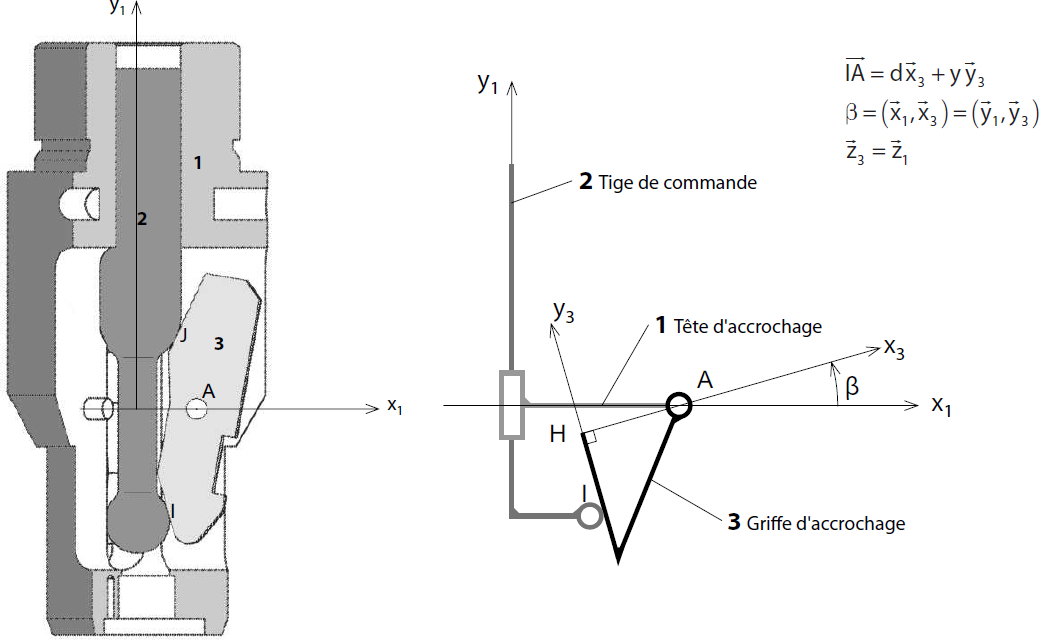
\includegraphics[width=\linewidth]{fig_01}
\end{marginfigure}


\section*{Mise en situation}
\ifprof
\else

\begin{marginfigure}
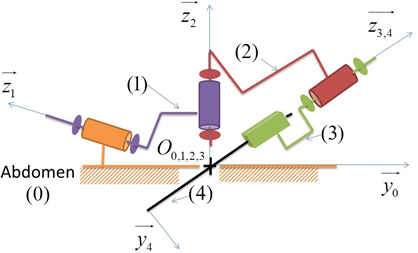
\includegraphics[width=\linewidth]{fig_02_a}
%\textit{}
\end{marginfigure}
Le robot $\text{MC}^2\text{E}$ est utilisé par des chirurgiens en tant que troisième main lors de l'ablation de la vésicule biliaire. La cinématique du robot permet de garantir que le point d'insertion des outils chirurgicaux soit fixe dans le référentiel du patient. 


\begin{marginfigure}
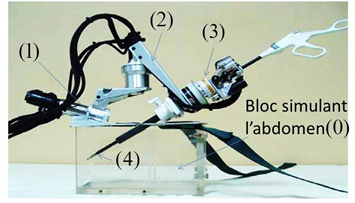
\includegraphics[width=\linewidth]{fig_02_b}
%\textit{}
\end{marginfigure}
Le robot est constitué de 3 axes de rotations permettant de mettre en position une pince. La pince est animée d'un mouvement de translation permettant de tirer la vésicule pendant que le chirurgien la détache du foie. 


On appelle trocart la pièce qui fait l'interface avec l'abdomen du patient et qui va guider l'ensemble des instruments. 

\begin{center}
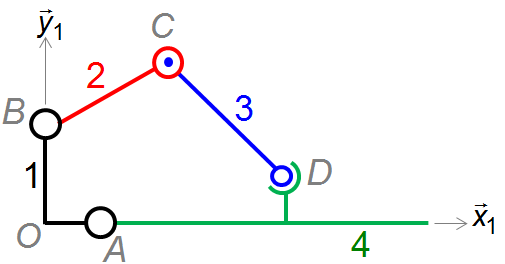
\includegraphics[width=\linewidth]{fig_09}
%\textit{}
\end{center}


La figure au verso donne un extrait du cahier des charges. 
%\begin{center}
%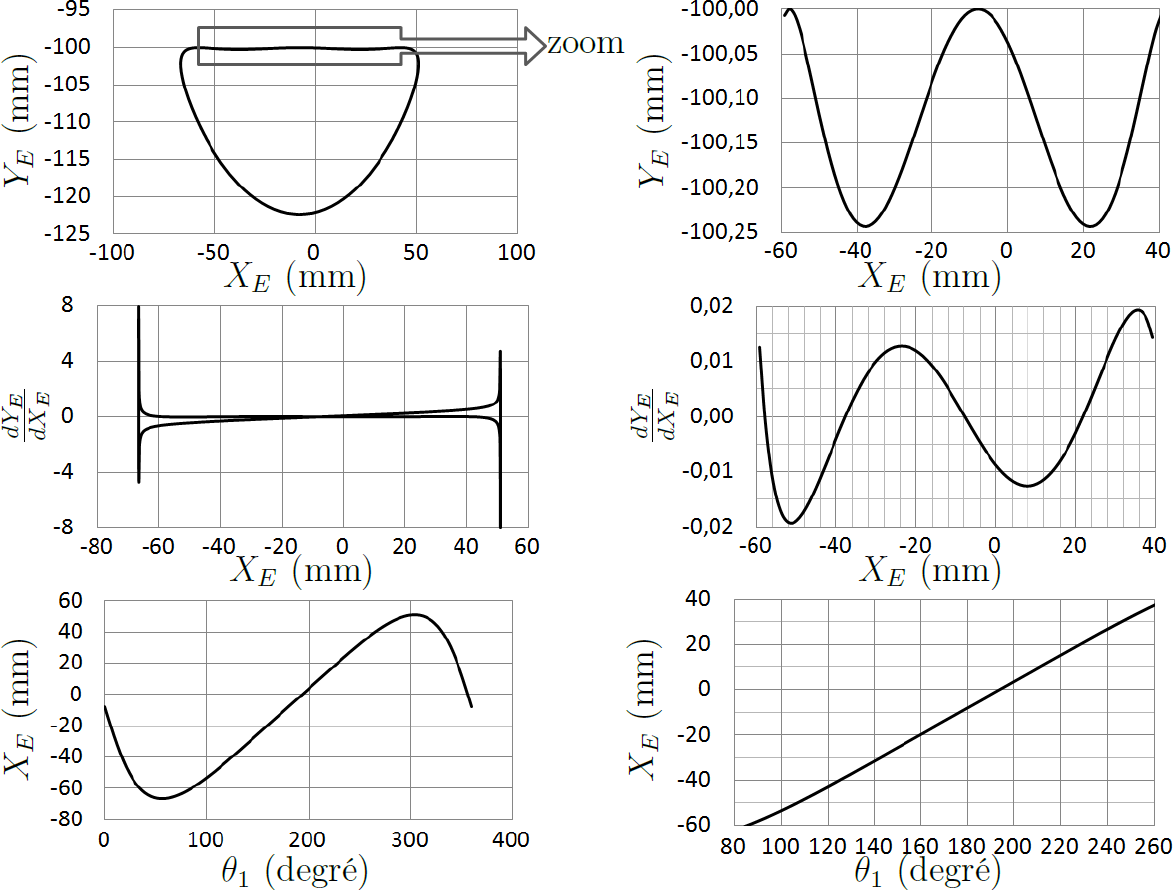
\includegraphics[width=\linewidth]{fig_03}
%%\textit{}
%\end{center}

\fi

\subsection*{Travail demandé}
\ifprof
\else
On s'intéresse à la phase de vie pendant laquelle la pince est introduite dans le trocart au travers d’un guide (étanche). Une phase de calibration du robot démarre ensuite. 
\begin{obj} ~\\
\vspace{-.5cm}
\begin{itemize}
\item Modéliser la liaison entre l’abdomen et la pince \textbf{(4)} en analysant la chaine ouverte de solides du robot.
\item Analyser les conséquences de la fermeture de la chaine par la liaison peau-trocart.
\end{itemize}
\end{obj}

\fi

\ifprof 
\else
Dans cette phase, la pince du $\text{MC}^2\text{E}$ est dans l’abdomen du patient, via le trocart. On souhaite étudier ici quelques aspects de la géométrie et de la cinématique du robot liés notamment à la nécessité que le point d’incision $O_0 =O_{0,1,2,3}$ soit un point fixe.

Le torseur cinématique du solide \textbf{(i)} par rapport au solide \textbf{(j)}, réduit en $P$, sera noté :

$\torseurcin{V}{i}{j}=\torseurl{\vecto{i}{j}}{\vectv{P}{i}{j}}{P}=\torseurcol{\omega_{xij}}{\omega_{yij}}{\omega_{zij}}{V_{xij}}{V_{yij}}{V_{zij}}{P,\vect{x_k},\vect{y_k},\vect{z_k}}$.

\textbf{Hypothèses}

\begin{itemize}
\item L’abdomen \textbf{(0)} est supposé fixe.
\item La pince \textbf{(4)} est déjà introduite dans l’abdomen \textbf{(0)} du patient.
\item Il n’y a pas encore de contact avec l’organe.
\end{itemize}


\begin{marginfigure}
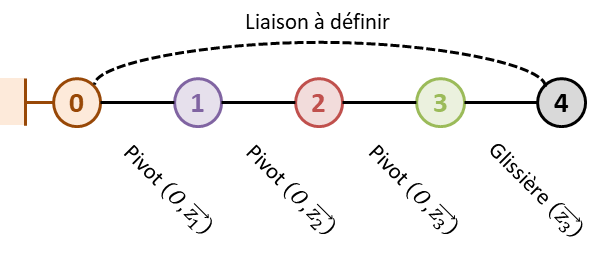
\includegraphics[width=\linewidth]{fig_10}
%\textit{}
\end{marginfigure}
On donne le graphe des liaisons du mécanisme ainsi modélisé.


La liaison entre la pince \textbf{(4)} et l’abdomen \textbf{(4)} n’est pas définie ici car elle est complexe : elle est notamment
imposée par la forme du trocart, que l’on suppose lié à l’abdomen du patient.
On va dans un premier temps considérer la chaîne ouverte de solides allant de \textbf{(0)} à \textbf{(4)} par l’intermédiaire des trois liaisons pivot et de la liaison glissière.
\fi

\question{On considère la chaîne ouverte de solides \textbf{(0+1+2+3+4)}. Par la méthode de votre choix, définir le torseur cinématique de la liaison équivalente 4/0 noté $\left\{\mathcal{V}^{\text{eq}}({4}/{0})\right\}$. En déduire la mobilité cinématique $m_c$
de cette chaîne de solides.}
\ifprof
\begin{corrige} ~\\
Les 4 solides étant en série, on a 
$\left\{\mathcal{V}^{\text{eq}}({4}/{0})\right\}=\torseurcin{V}{4}{3}+\torseurcin{V}{3}{2}+\torseurcin{V}{2}{1}+\torseurcin{V}{1}{0}$.
$O$ étant le point de concours de chacun des axes, les torseurs des liaisons pivots sont tous de la forme : 
$\torseurcin{V}{i}{i-1}=\torseurl{\dot{\theta}_i\vect{z_i}}{\vect{0}}{O}$.De plus,  $\torseurcin{V}{4}{3}=\torseurl{\vect{0}}{\dot{\lambda}\vect{z_3}}{O}$. 

Au final, $\left\{\mathcal{V}^{\text{eq}}({4}/{0})\right\}=\torseurl{\dot{\theta}_1\vect{z_1}+\dot{\theta}_2\vect{z_2}+\dot{\theta}_3\vect{z_3}}{\dot{\lambda}\vect{z_3}}{O}$.
 
 Il s'agit d'une liaison sphère-cylindre(linéaire annulaire) d'axe $\axe{O}{z_3}$. En conséquences $m_c=4$.
\end{corrige}
\else
\fi

\ifprof
\else

On envisage deux modélisations pour la liaison entre la pince \textbf{(4)} et la peau de l’abdomen par l’intermédiaire du trocart :
\begin{itemize}
\item modélisation 1 : liaison sphère-cylindre en $O_0$ d’axe $\axe{O_0}{z_3}$;
\item modélisation 2 : liaison libre : pas de liaison entre le bâti et la pince.
\end{itemize}

\fi

\question{Dans le cadre des deux modélisations retenues, quels sont alors le degré d’hyperstatisme et la mobilité cinématique de la chaîne fermée. Compléter le tableau du document réponse concernant les
implications du modèle retenu sur le robot et les interactions patient / robot. Quelle modélisation vous
parait la plus proche de la réalité ? Argumenter votre réponse.}

\ifprof


\begin{corrige} ~\\
\footnotesize
\begin{center}
\begin{tabular}{|p{2.2cm}|p{2cm}|p{2cm}|}
\hline
& Liaison linéaire annulaire & Liaison libre  \\
\hline
$m_c=$ & 4 & 4\\ \hline
$h=$ & $m-I_c+E_c = 4 - (4+4) + 6 = 2$ &0 (Chaîne ouverte)\\ 
$h=$ & $m-E_s+I_s = 4 - 24 + 22 = 2$ &0 (Chaîne ouverte)\\ 
% & & \\ 
 \hline
Efforts au point d'insertion* & Oui (à cause de l'hyperstatisme)& Non \\ \hline
Facilité de montage ?* & Non (à cause de l'hyperstatisme)& Oui \\ \hline
Rigidité du robot* & Oui... &  Oui...\\ \hline
\multicolumn{3}{c}{\textit{* : Remplir par oui ou non}}
\end{tabular}
\end{center}
\normalsize
Les réponses données dans le tableau sont qualitative et critiquable... L'hyperstatisme impose des contraintes dans la fabrication l'assemblage du robot qui peuvent se traduire par des efforts à <<vaincre>> lors de l'assemblage ou de la mise en position du robot. 

Un système hyperstatique est réputé plus rigide qu'un système isostatique. Cependant, lorsqu'un système est isostatique, sans jeu et avec des frottements, on peut aussi le considérer comme étant rigide...
\end{corrige}
\else


\footnotesize
\begin{center}
\begin{tabular}{|p{2.2cm}|p{2cm}|p{2cm}|}
\hline
& Liaison linéaire annulaire & Liaison libre  \\
\hline
$m_c=$ & & \\ \hline
$h=$ & & \\ \hline
Efforts au point d'insertion* & & \\ \hline
Facilité de montage ?* & & \\ \hline
Rigidité du robot* & & \\ \hline
\multicolumn{3}{c}{\textit{* : Remplir par oui ou non}}
\end{tabular}
\end{center}
\normalsize
%\end{corrige}
\fi


\subsection*{Retour sur le cahier des charges}


\question{Quelle exigence le mécanisme utilisé permet-il de satisfaire ? Expliquer en 2 lignes comment cette exigence est satisfaite. }

\ifprof
\begin{corrige}~\\
La structure du robot permet de satisfaire l'exigence 1.3 : <<~Ne pas endommager l'abdomen du patient~>>. En effet, le fait que les axes des 3 pivots s'intersectent en un point permet d'avoir un seul point d'entrée de la pince dans l'abdomen. Ainsi, on diminue les risques de <<~blesser~>> davantage le patient lors de l'opération de la vésicule. 
\end{corrige}
\else
\fi


\ifprof
\else
\ifcolle
\else
\begin{marginfigure}[-4cm]
\begin{solution}
\begin{enumerate}
\item Liaison sphère cylindre d'axe $\axe{O}{z_3}$.
\item Cas 1 : $m_c=4$, $h=2$. Cas 2 : $m_c=4$, $h=0$.
\item Exigence 1.3.
\end{enumerate} 
\end{solution}
\end{marginfigure}
\fi
\fi
\normalsize


\ifprof
\else


\begin{center}
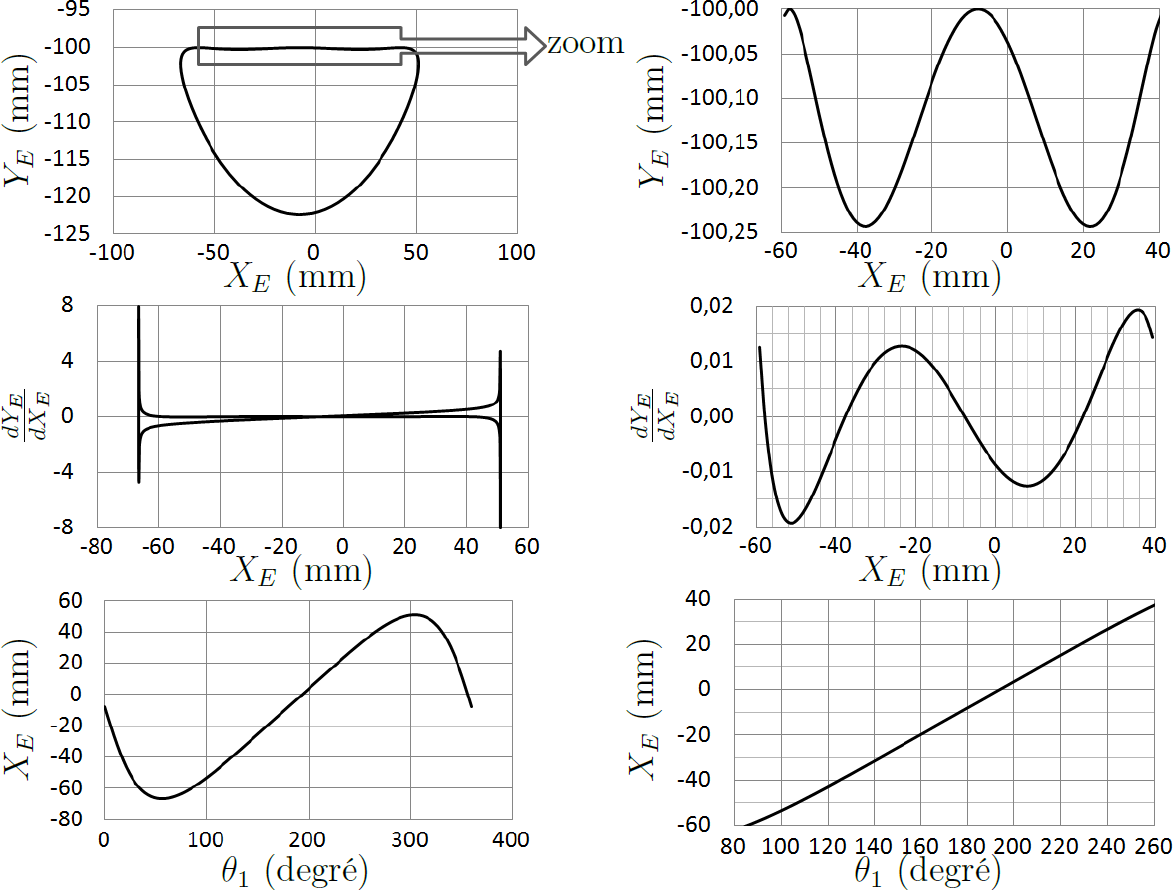
\includegraphics[width=\linewidth]{fig_03}
%\textit{}
\end{center}
\fi
%\begin{center}
%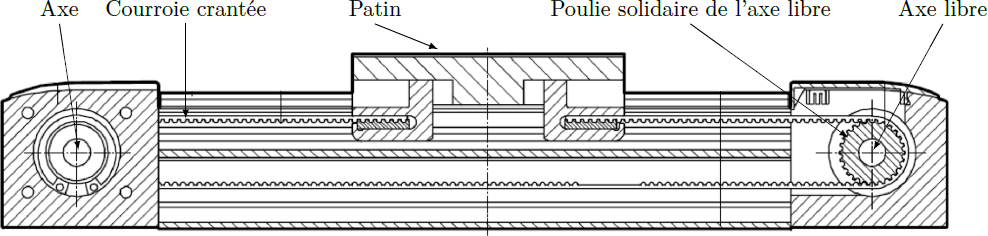
\includegraphics[width=\linewidth]{fig_04}
%%\textit{}
%\end{center}

